\subsection{Analysis of Activity Estimates}

Density and abundance estimates obtained using distance estimates generated with each
configuration of the distance estimation pipeline for both the supplemented data (manual
frame sample) and model only data (automated frame sample) are shown in
Figure~\ref{fig:activity_chart}.

\begin{figure}[H]
    \vspace{1cm}
    \centering
    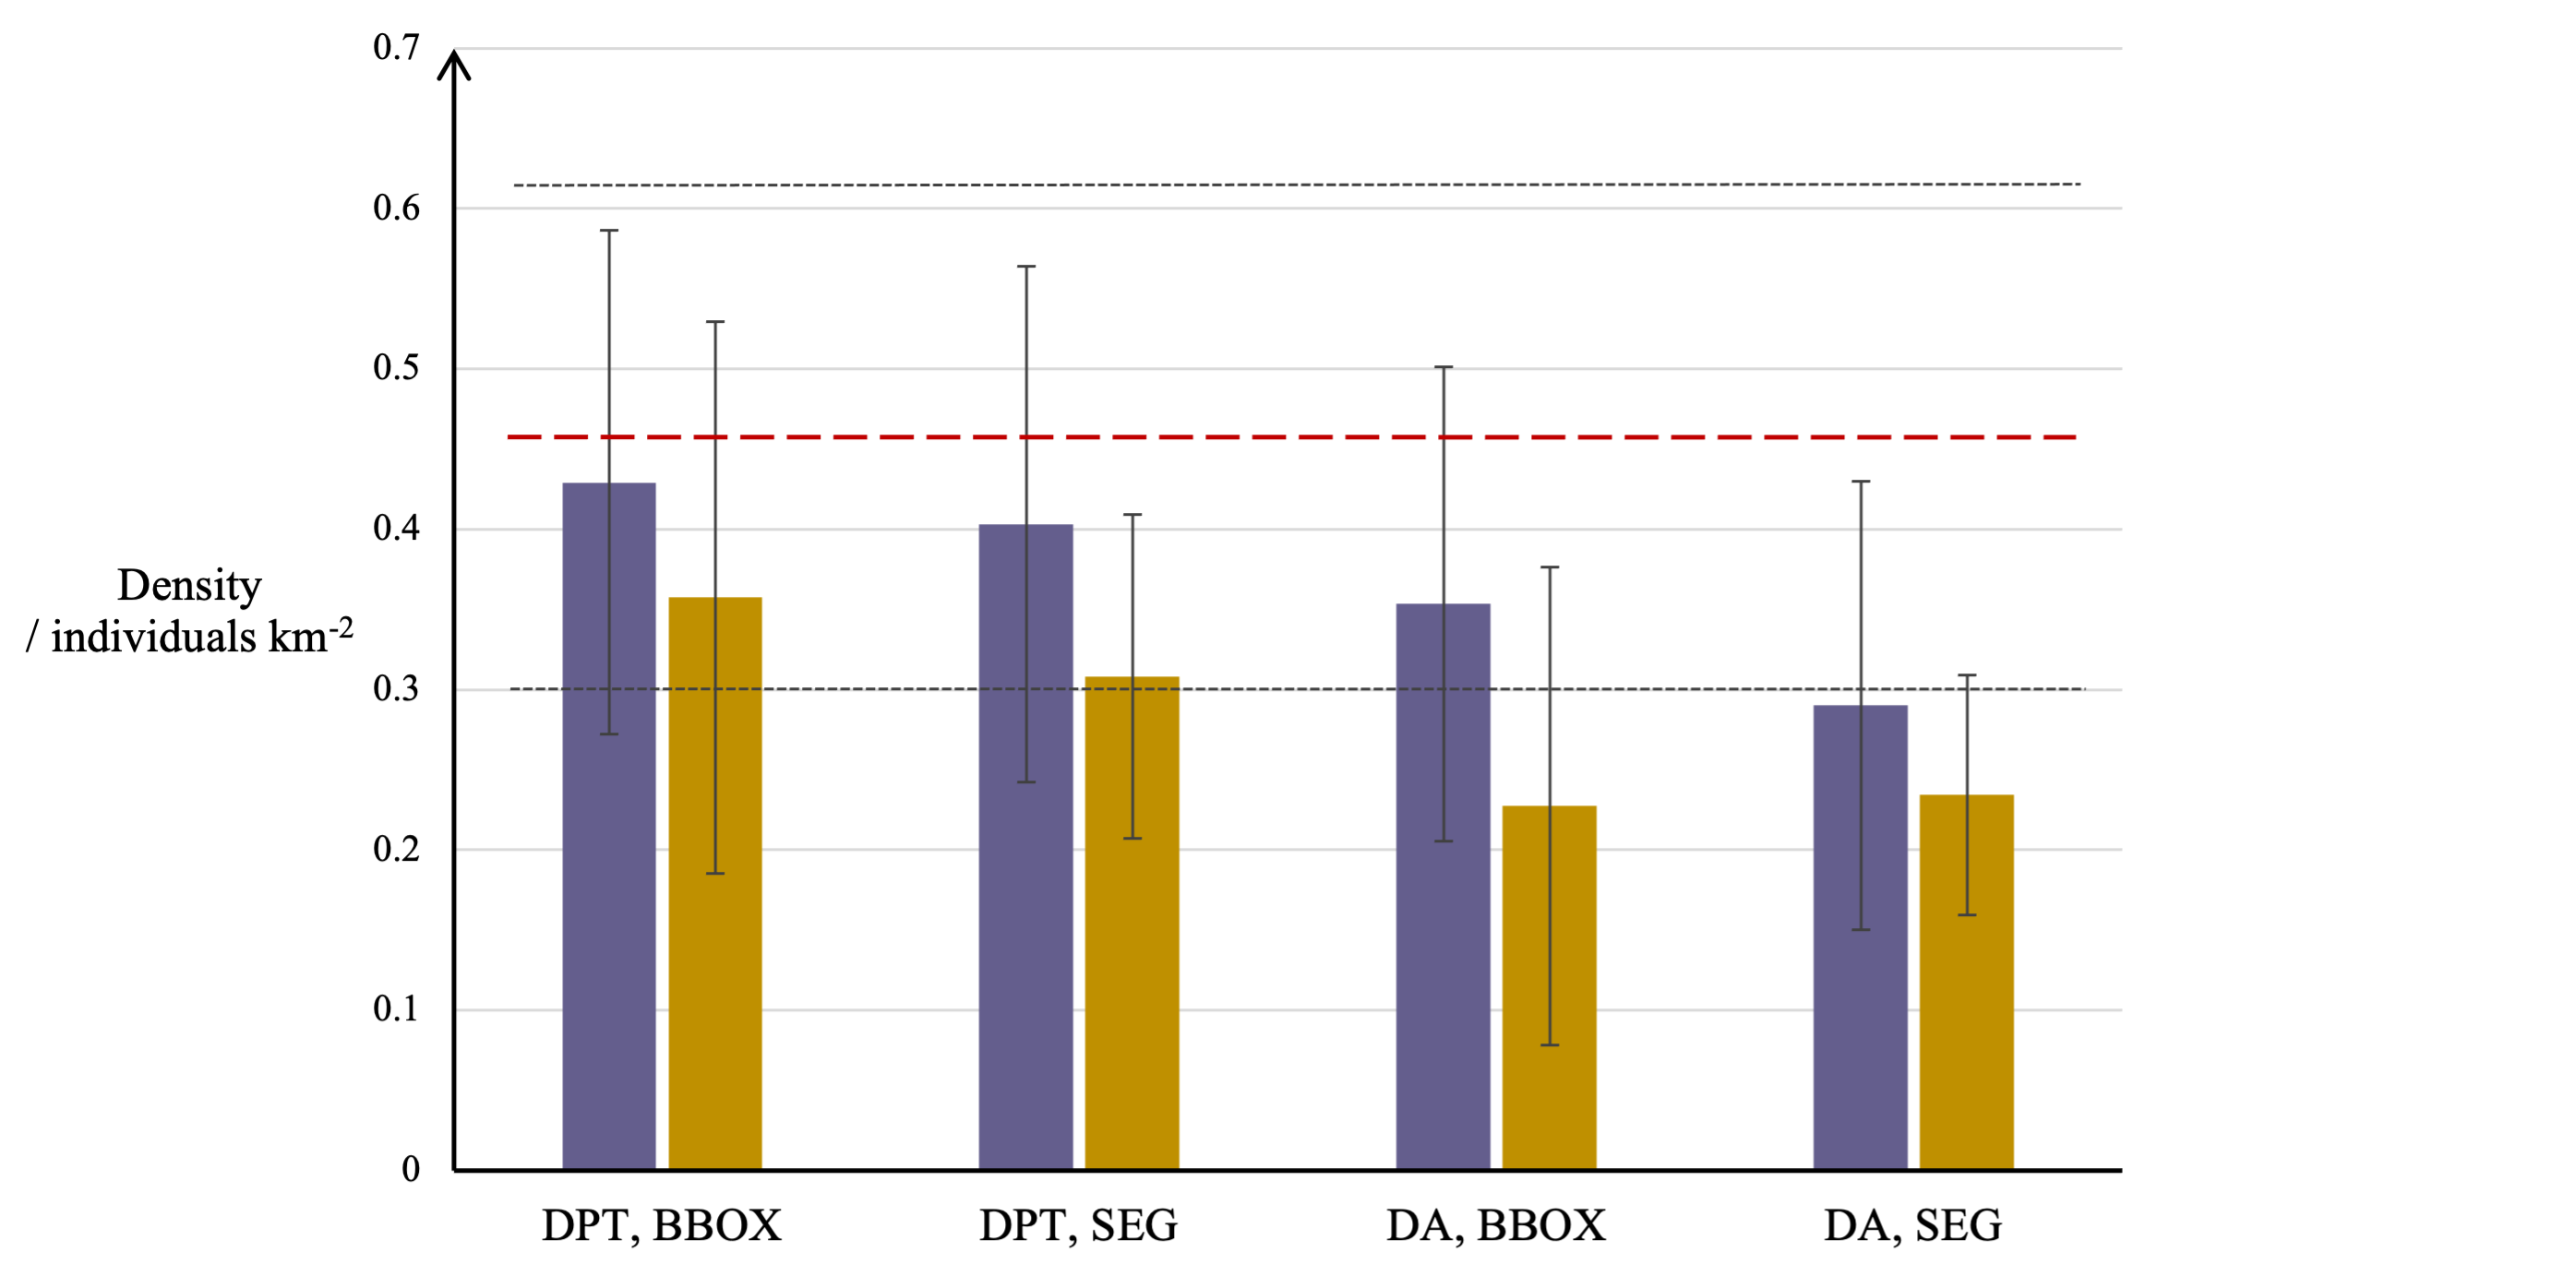
\includegraphics[width=0.8\textwidth]{body/analysis/assets/activity/density_chart}
    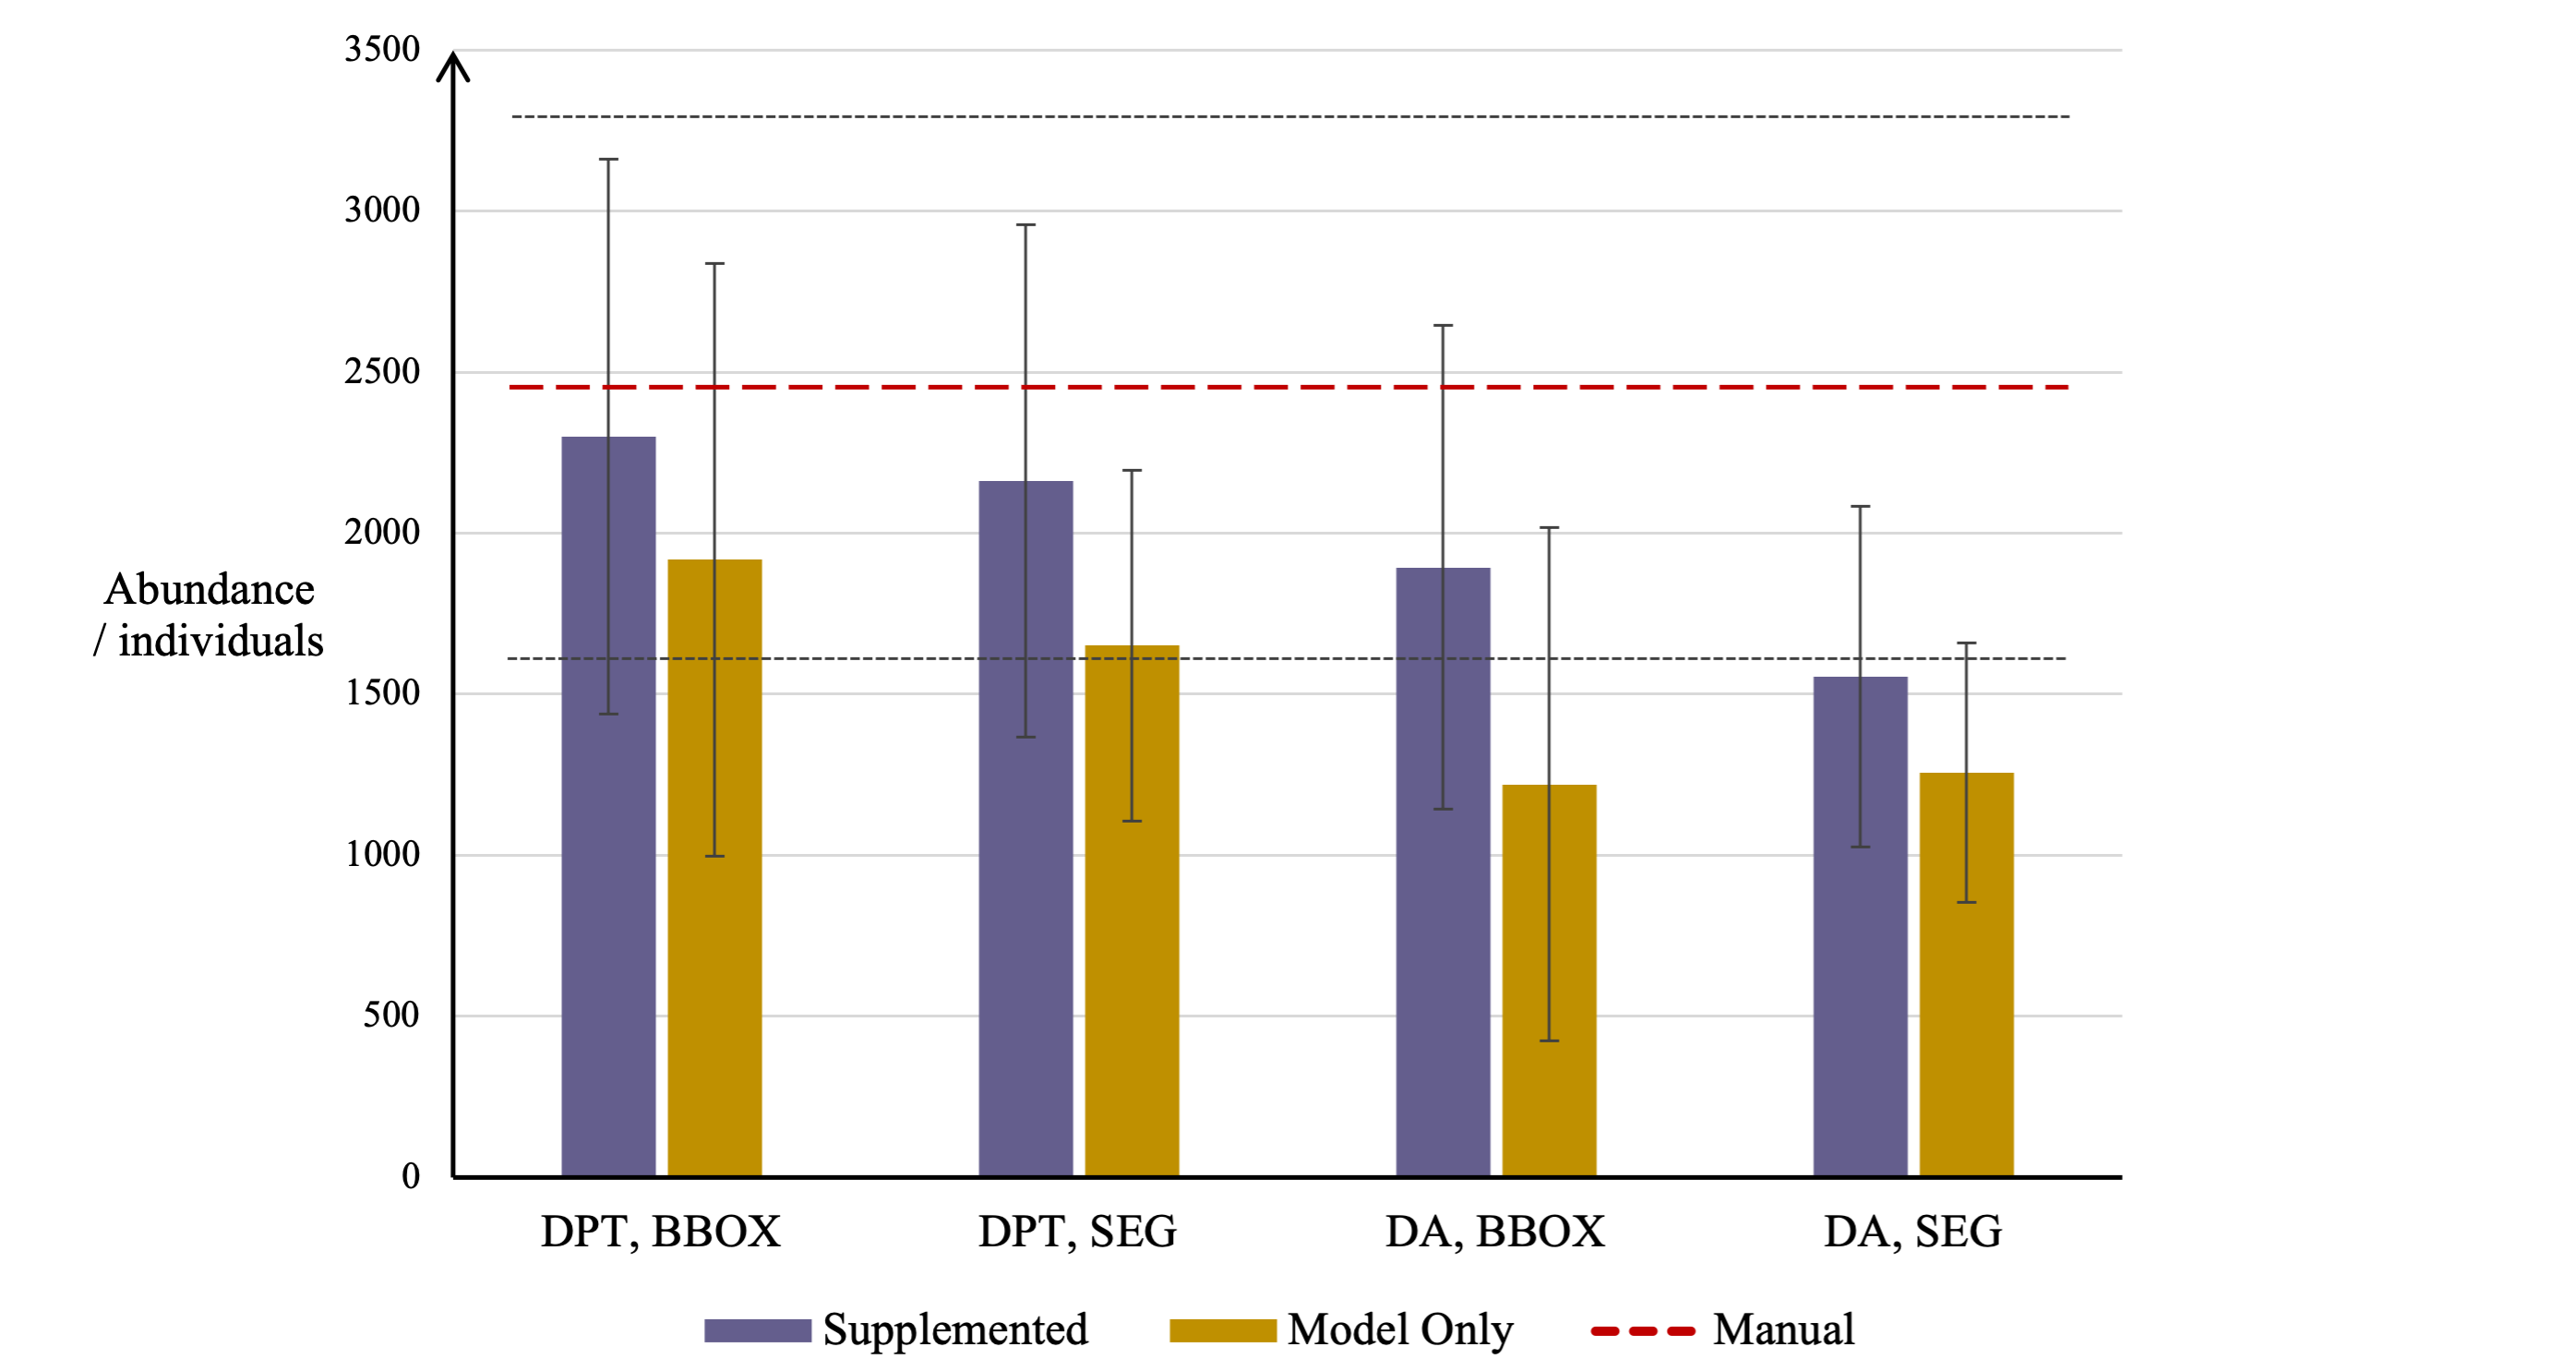
\includegraphics[width=0.81\textwidth]{body/analysis/assets/activity/abundance_chart}
    \caption{Density (top) and abundance (bottom) estimates for the chimpanzee population
        (Taï national park), derived with camera trap video from the WCF dataset.
        Estimates are given using distance estimates obtained from each configuration of the
        distance estimation pipeline with both the manual sample (Supplemented) and automated
        sample (Model Only). The error bars show the standard error corresponding to
        each configuration. The density and abundance estimates given by the manually estimated
        distances are shown with the red dashed lines and the errors by the grey dashed lines.}
    \label{fig:activity_chart}
\end{figure}

\subsubsection{Configuration Effects}



\subsubsection{Sample Effects}

Single chimp frame distances supplemented with manual distances

\subsubsection{Additional Considerations}

False Positives and Misses
